\PassOptionsToPackage{dvipsnames}{xcolor}
% \documentclass[handout]{beamer}
\documentclass{beamer}
\usepackage{xcolor}
\usetheme[background=light,block=fill,]{metropolis} % Use metropolis theme
% \usetheme{Madrid}
\usepackage{amsmath,amssymb,amsfonts,amsthm,mathtools}

\title{Evil Rings}
\subtitle{\footnotesize Not All Rings Are Round: A Journey Through Misfit Math}
\date{August 28, 2024}
\author{Aryaman Maithani}
\institute{University of Utah}

\usepackage{parskip}
\usepackage[
	hyperref = true,      	% Link to online documents
  	backend  = bibtex,      % Use bibtex instead of biber
  	sorting  = nyt,       	% Sorts by (name, year, title)
  	style  = alphabetic, 	% Citations look like [Har77]
  	maxbibnames = 5,
  	doi=false,isbn=false,url=false,eprint=false
]{biblatex}
\addbibresource{talks.bib}

\newtheorem{punchline}[theorem]{Punchline}
\newtheorem{punchlines}[theorem]{Punchlines}
\newcommand{\limit}{\varprojlim}
\newcommand{\md}[1]{{\left\lvert #1 \right\lvert}}
\DeclareMathOperator{\htt}{height}
\DeclareMathOperator{\Sing}{Sing}
\DeclareMathOperator{\Spec}{Spec}
\DeclareMathOperator{\Frac}{Frac}
\DeclareMathOperator{\pdim}{pdim}
\DeclareMathOperator{\depth}{depth}

\usepackage{hyperref}
\hypersetup{
	colorlinks = true,
	linkcolor = BrickRed,
	citecolor = Green,
	% urlcolor   = blue
  	filecolor = red
}

\begin{document}
	\maketitle

	\begin{frame}{Conventions}
		All rings mentioned will be commutative and unital. \pause \newline
		\phantom{h} \hfill {\tiny (Nonunital rings might just be too evil...)} \pause

		Depending on your taste, you may think that any nonnoetherian ring is evil. \pause We will look at some examples of strange behaviour of nonnoetherian rings, but then stick to noetherian rings for the majority of the talk.
	\end{frame}

	\begin{frame}{One mathematician's pathology is another's normalcy}
		Such a talk if of course subjective. For example, ChatGPT \cite{ChatGPT} suggested the following (\emph{surely} benign) rings as evil. \pause

		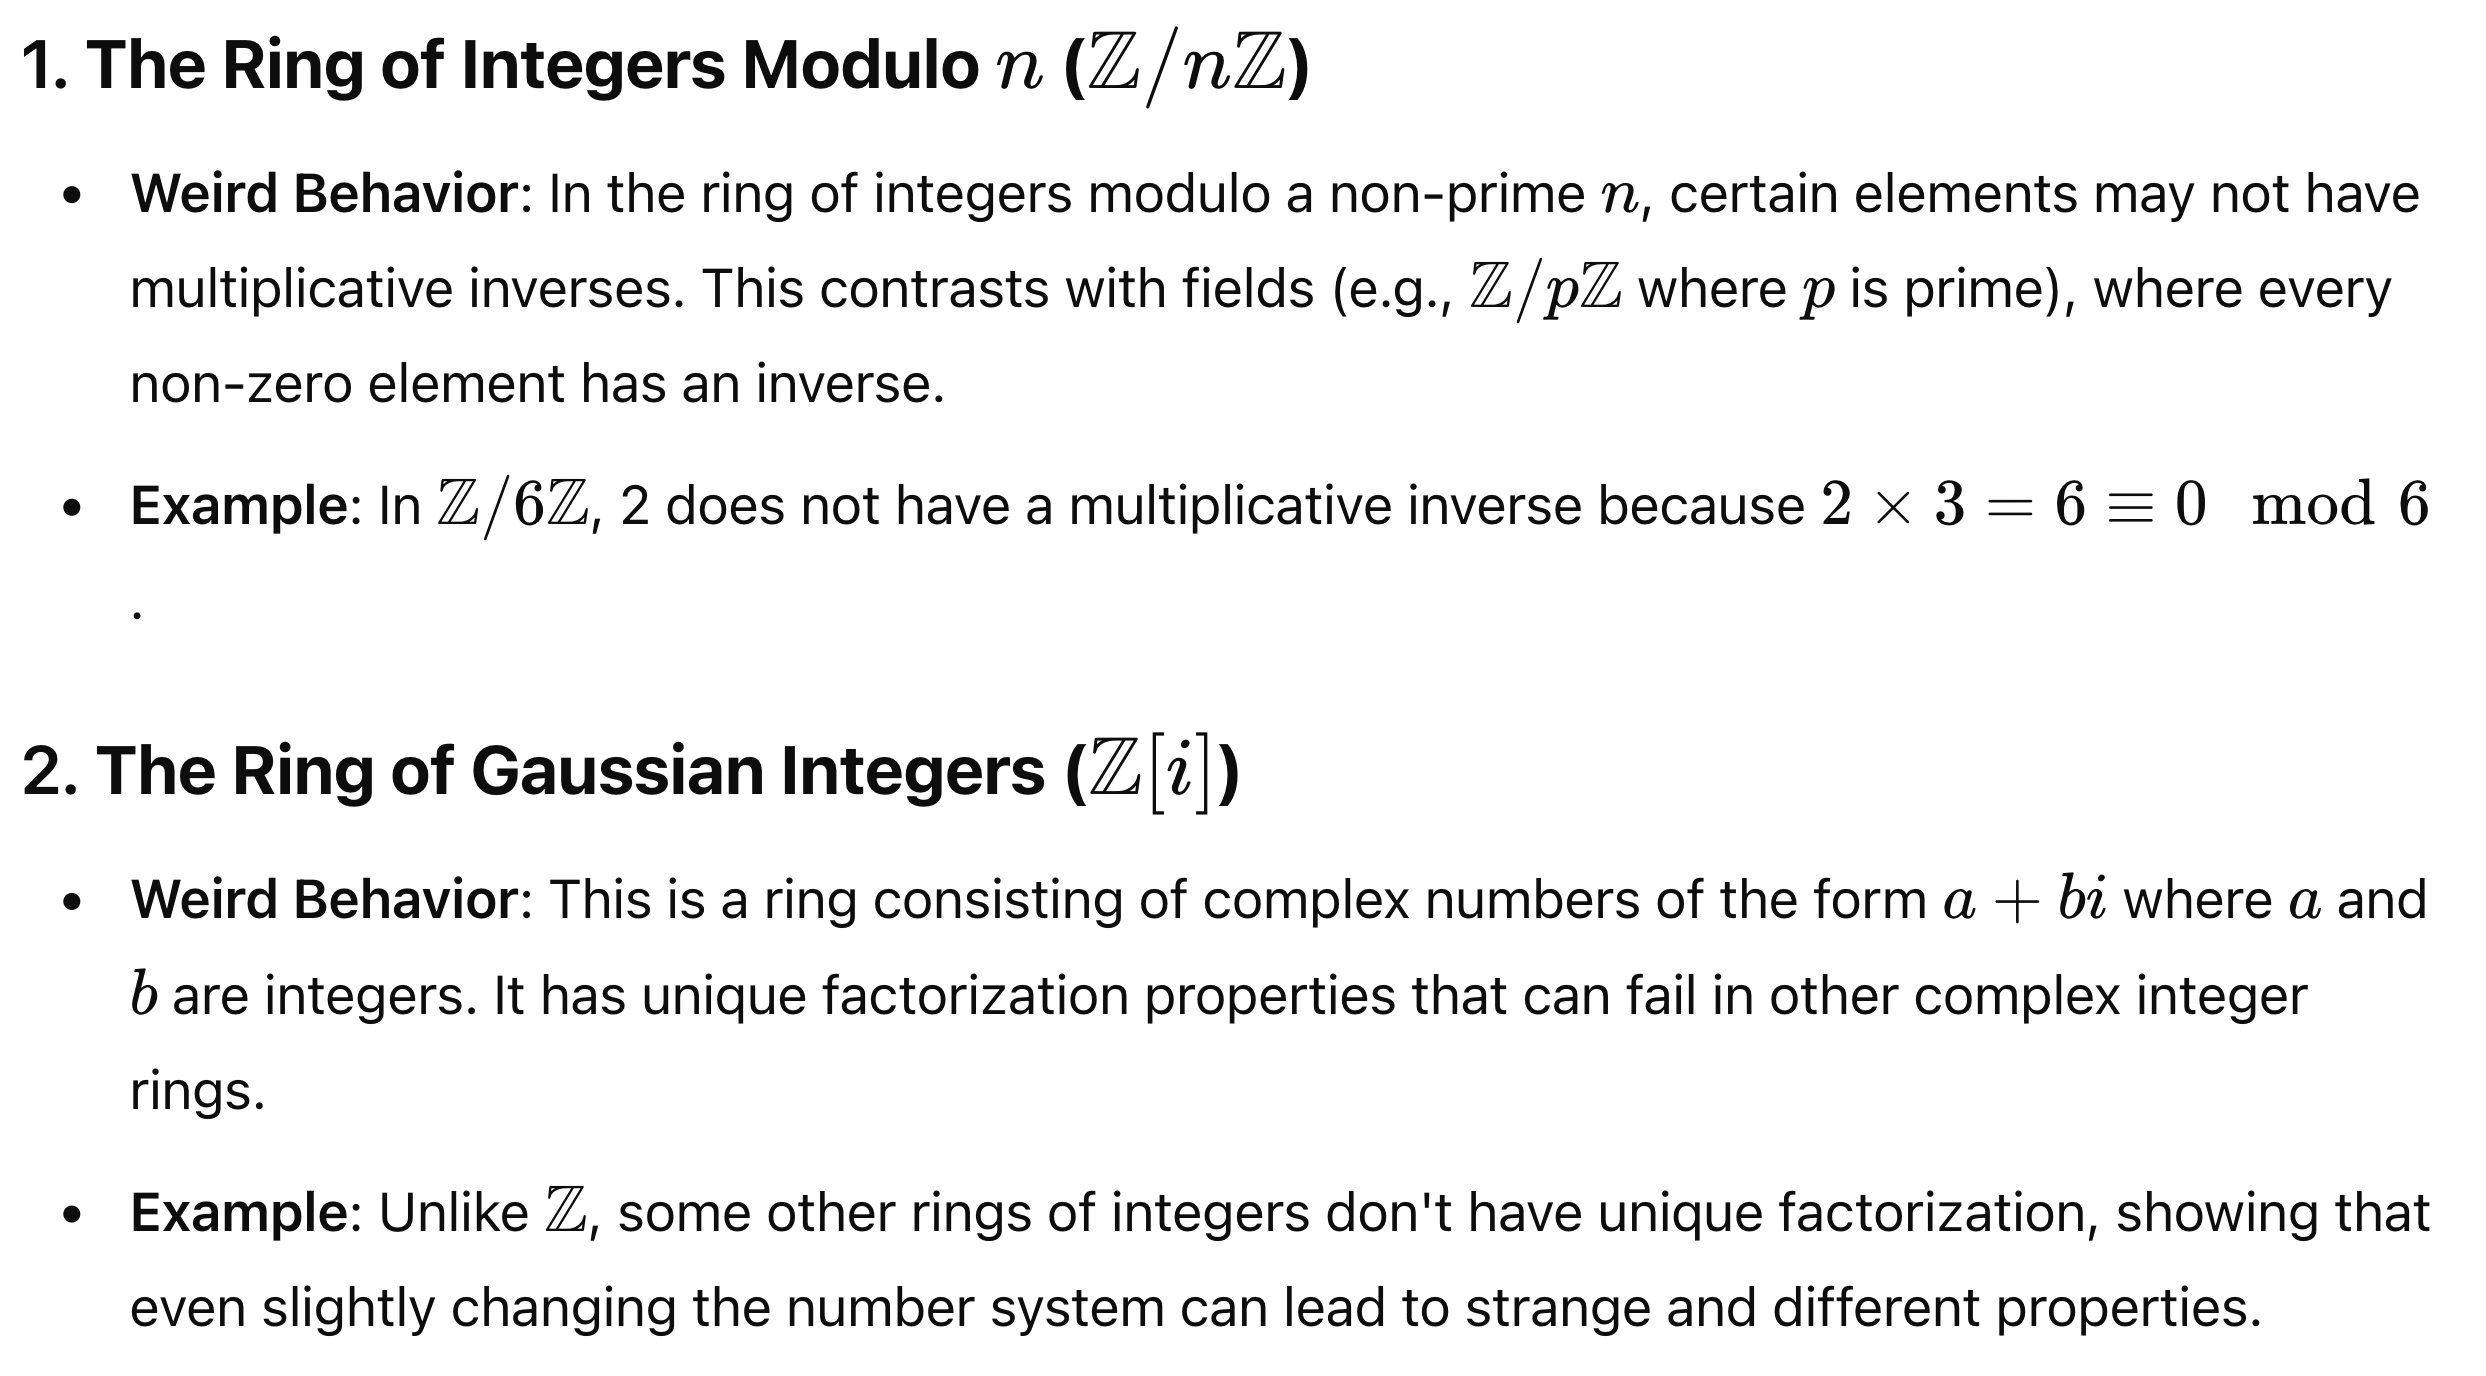
\includegraphics[width=\textwidth]{figs/chat-gpt-evil.png}
	\end{frame}

	\begin{frame}{Tensoring noetherian algebras}
		Have you thought about $k[\![x]\!] \otimes_{k} k[\![y]\!]$? \pause This is \emph{not} $k[\![x, y]\!]$. \pause In fact: 
		\begin{punchline}
			Each of the following rings is not noetherian: \pause $k[\![x]\!] \otimes_{k} k[\![y]\!]$, \pause $k[\![x]\!] \otimes_{k} k(\!(y)\!)$, \pause and $k(\!(x)\!) \otimes_{k} k(\!(y)\!)$.
		\end{punchline} % ??
	\end{frame}

	\begin{frame}{Krull's height theorem}
		Krull's principal ideal theorem states: in a noetherian ring, every minimal prime over a proper {\color{Red}principal} ideal \pause has height at most {\color{Red}one}. \pause

		This fails in every valuation domain $(R, \mathfrak{m})$ with dimension at least two: \pause pick a prime $\mathfrak{p}$ strictly between $0$ and $\mathfrak{m}$. \pause Pick $x \in \mathfrak{m} \setminus \mathfrak{p}$. \pause Since ideals in a valuation domain are linearly ordered, we get
		\begin{equation*} 
			0 \subsetneq \mathfrak{p} \subsetneq (x) \subseteq \mathfrak{m}.
		\end{equation*} \pause
		Any minimal prime over $(x)$ has height at least two. \pause

		{\tiny Such valuation domains do exist!}
	\end{frame}

	\begin{frame}{Incomplete completions}
		Let $R$ be a ring and $\mathfrak{m}$ a maximal ideal. \pause The \emph{completion} of $R$ (with respect to $\mathfrak{m}$) is defined as 
		\begin{equation*} 
			\widehat{R} = \limit R/\mathfrak{m}^{n}.
		\end{equation*} \pause
		The following is true: $\widehat{R}$ is a local ring with unique maximal ideal $\mathfrak{M} \coloneqq \ker(\widehat{R} \to R/\mathfrak{m})$. \pause

		\begin{punchlines}
			All of the following have negative answers: \pause \newline
			Is $\mathfrak{m} \widehat{R} = \mathfrak{M}$? \pause \newline
			Is $\widehat{R}$ viewed as an $R$-module $\mathfrak{m}$-adically completely? \pause \newline
			Is $\widehat{R}$ viewed as an $\widehat{R}$-module $\mathfrak{M}$-adically completely, i.e., is $\widehat{R}$ a complete local ring? 
		\end{punchlines} \pause
		$R = k[x_{1}, x_{2}, \ldots]$ and $\mathfrak{m} = (x_{1}, x_{2}, \ldots)$ serve as a uniform (counter)example. \hfill {\footnotesize \cite[\href{https://stacks.math.columbia.edu/tag/05JA}{Tag 05JA}]{stacks-project}}
	\end{frame}

	\begin{frame}{Turbulence over...}
		Rings in the forthcoming slides will all be noetherian!
	\end{frame}

	\begin{frame}{Revisiting Krull's height theorem}
		Krull was the first to show that a great deal of the geometric theory of the polynomial ring could be carried over to the noetherian case, \pause indicating that is a good class of rings to work with. \pause

		The Krull dimension of a ring can be defined as the supremum of heights of all of its prime ideals. \pause By Krull's height theorem, we see that every prime ideal in a noetherian ring has finite height. \pause In particular, noetherian local rings have finite dimension. \pause

		\textbf{Question.} Does there exist a noetherian ring with infinite Krull dimension?
	\end{frame}

	\begin{frame}{Nagata's example}
		\vphantom{H}

		\begin{punchline}[Nagata]
			There exists a noetherian domain with infinite Krull dimension.
		\end{punchline} 
		\pause
		Construction: Consider the polynomial ring in $\omega$-many variables: \pause
		% \begin{align*} 
		{\centering
		$
			\begin{aligned}
				R \coloneqq k[&x_{11}, \\
				& x_{21}, x_{22}, \\
				& x_{31}, x_{32}, x_{33}, \ldots]. 
			\end{aligned}
		$
		\par}
		% \end{align*}
		\pause 
		For $n \ge 1$, define the prime ideal $\mathfrak{p}_{n} \coloneqq (x_{n1}, \ldots, x_{nn})$ \pause and set $W \coloneqq R \setminus \bigcup_{n \ge 1} \mathfrak{p}_{n}$. \pause 

		Then, $S \coloneqq W^{-1} R$ is a noetherian domain whose maximal ideals are $W^{-1}\mathfrak{p}_{n}$. \pause As $\htt(W^{-1} \mathfrak{p}_{n}) = n$, we see that $\dim(S) = \infty$. \qed \pause

		{\footnotesize This was Nagata's original example given in \cite[Appendix A1]{NagataLocalRings}.}
	\end{frame}
	\begin{frame}{Nagata's example continued}
		Moreover, observe that the localisation of $S$ at each maximal ideal is regular and thus, $S$ is itself a regular domain. \pause In particular, $S$ is also Gorenstein but has infinite injective dimension. \pause This gives us:

		\begin{punchline}
			There exists a Gorenstein ring with infinite injective dimension.
		\end{punchline} 
	\end{frame}

	\begin{frame}{Excellent rings}
		The definition of an \emph{excellent} ring is available at \url{https://en.wikipedia.org/wiki/Excellent_ring}. \pause This is considered a ``well-behaved'' class of rings to work with. \pause Most naturally occurring commutative rings in number theory or algebraic geometry are excellent. \pause Such rings are noetherian, \pause universally catenary, \pause have finite Krull dimension, \pause have a closed singular locus, ... \pause

		The \emph{singular locus} of a ring $R$ is 
		\begin{equation*} 
			\Sing(R) \coloneqq \{\mathfrak{p} \in \Spec(R) : R_{\mathfrak{p}} \text{ is not regular}\}.
		\end{equation*} \pause
		Note: If $\Sing(R) = V(\mathfrak{a})$, then any $f \in \mathfrak{a} \setminus \{0\}$ has the property that $R_{f}$ is regular. \pause \newline
		Moreover, if $R$ is a domain, then $\mathfrak{a} \neq (0)$.
	\end{frame}
	\begin{frame}{Non-excellent noetherian rings}
		Our previous example was infinite-dimensional and hence, not excellent. \pause Thus, there exist nonexcellent noetherian rings. \pause Another example is furnished with the following.
		\begin{punchline}
			There exists a noetherian domain whose singular locus is not closed.
		\end{punchline} \pause
		Construction: Consider $R \coloneqq k[x_{1}^{2}, x_{1}^{3}, x_{2}^{2}, x_{2}^{3}, \ldots]$, \pause $\mathfrak{p}_{n} \coloneqq (x_{n}^{2}, x_{n}^{3})$, \pause $W \coloneqq R \setminus \bigcup_{n \ge 1} \mathfrak{p}_{n}$, \pause and $S \coloneqq W^{-1} R$. \pause $S$ is noetherian for similar reasons as before. \pause

		Note that $S_{\mathfrak{p}_{n} S}$ is not normal and hence not regular. \pause Every nonzero element avoids some $\mathfrak{p}_{n}$. \pause Thus, $S_{f}$ is not regular for any $f \in S \setminus \{0\}$. \pause Since $S$ is a domain, this shows that $\Sing(S)$ is not closed. \qed
	\end{frame}

	\begin{frame}{Projective dimensions}
		Consider $R \coloneqq \mathbb{R}[x, y, z]$. \pause This ring has global dimension $3$, \pause this means that that \underline{every} $R$-module has a projective resolution of length (at most) $3$. \pause Consider $Q \coloneqq \Frac(R)$ as a module over $R$. \pause

		What is $\pdim_{R}(Q)$? \pause %That is, what is the shortest length of an $R$-projective resolution of $Q$? \pause

		\begin{theorem}[Osofsky \cite{OsofskyCH}]
			The following are equivalent: \pause
			\begin{itemize}[<+->]
				\item $\pdim_{R}(Q) = 2$.
				\item The continuum hypothesis holds. 
			\end{itemize}
		\end{theorem}

		\phantom{h} \hfill {\tiny Try running \emph{this} on M2...}
	\end{frame}

	\begin{frame}{Are complete intersections complete intersections?}
		Recall that a local ring $R$ is defined to be a \emph{complete intersection} if \pause
		\begin{equation*} 
			\widehat{R} \cong \dfrac{\text{regular local ring}}{(\text{regular sequence})}.
		\end{equation*} \pause
		\textbf{Question.} Is every c.i. $R$ itself a quotient of the above form? \pause

		\begin{punchline}[Heitmann--Jorgensen]
			There exists a three-dimensional complete intersection domain which is not a homomorphic image of a regular local ring.
		\end{punchline} \pause

		This is from the paper \emph{``Are complete intersections complete intersections?''} \cite{HeitmannJorgensen}, that has an example where the completion is $\mathbb{R}[\![x, y, z, w]\!]/(x^{2} + y^{2})$.	
	\end{frame}
	\begin{frame}{Lack of imagery}
		The previous example was from 2011. \pause In 1978, one knew: \pause
		\begin{punchlines}[Marinari] 
			There exists a one-dimensional local Gorenstein domain which is not a homomorphic image of a regular local ring. \pause

			There exists a one-dimensional local Cohen--Macaulay domain which is not a homomorphic image of a Gorenstein ring. 
		\end{punchlines} \pause
		These examples were constructed in the paper \emph{``Examples of bad Noetherian local rings''} \cite{MarinariBadNoetherian} \pause using a technique attributed to Larfeldt--Lech \cite{LarfeldtLech}. \pause \newline
		For a Cohen--Macaulay ring, being the image of a Gorenstein ring is equivalent to possessing a canonical module. \pause Thus, the above shows that there exist CM rings without canonical modules.
	\end{frame}
	\begin{frame}{UFD + CM \texorpdfstring{$\Rightarrow$}{=>} G?}
		% https://www.math.purdue.edu/~jlipman/papers-older/%5B1975%5D%20Unique%20factorization%20in%20complete%20local%20rings.pdf
		 \pause Murthy \cite{MurthyUFD} showed that a Cohen--Macaulay UFD possessing a canonical module is Gorenstein. \pause
		\begin{punchline}
			There exists a two-dimensional UFD ($\Rightarrow$ CM) which is not a Gorenstein ring.
		\end{punchline} \pause
		Such a ring is thus not the image of a Gorenstein ring.
	\end{frame}
	\begin{frame}{UFD \texorpdfstring{$\Rightarrow$}{=>} CM?}
		% https://www.math.purdue.edu/~jlipman/papers-older/%5B1975%5D%20Unique%20factorization%20in%20complete%20local%20rings.pdf
		For a while, the question ``UFD $\Rightarrow$ CM?'' was open under various contexts. \pause 

		\begin{punchlines}
			There exists a local UFD which is not Cohen--Macaulay. \pause

			There exists a complete local UFD which is not Cohen--Macaulay. 
		\end{punchlines} \pause
		Examples for both can be obtained via invariant subrings: \pause Consider the action of $G \coloneqq \mathbb{Z}/4$ on $S \coloneqq \mathbb{F}_{2}[w, x, y, z]$ by cyclically permuting the variables. \pause The fixed subring $R \coloneqq S^{G}$ is a (graded) UFD which is not CM. \pause Localising and completing at the homogeneous maximal yields the examples. \newline
		\phantom{h} \hfill {\footnotesize See \cite[\S4]{LipmanUFDs} for a discussion.}
	\end{frame}

	\begin{frame}{Characterising completions: Lech}
		Lech's \emph{``A Method for Constructing Bad Noetherian Local Rings''} \cite{LechBadNoetherianLocal} characterises what rings can be obtained as the completion of a noetherian local domain. \pause

		A corollary: if $S$ is a complete noetherian local ring \pause containing a field \pause and $\depth(S) \ge 1$, then $S$ can be obtained so. \pause

		Thus, there exists a noetherian local domain $R$ such that $\widehat{R} \cong \mathbb{C}[\![x, y]\!]/(x^{2})$; \pause this is not reduced.
	\end{frame}
	\begin{frame}{Characterising completions: Heitmann}
		Similarly, Heitmann \cite{HeitmannCharacterizeUFDCompletion} characterised in 1993 which rings can be obtained as the completion of a local UFD. \pause 

		A corollary: if $S$ is a complete noetherian local ring containing a field and $\depth(S) \ge 2$, then $S$ can be obtained so. \pause

		Jacking up the previous example, there exists a noetherian local UFD $R$ such that $\widehat{R} \cong \mathbb{C}[\![x, y, z]\!]/(x^{2})$; this is again not reduced.
	\end{frame}

	\begin{frame}{Catenary}
		A ring is \emph{catenary} if for any pair of prime ideals $\mathfrak{p}$, $\mathfrak{q}$, \pause any two maximal chains of primes from $\mathfrak{p}$ to $\mathfrak{q}$ \pause have the same length. \pause % The ring is \emph{universally catenary} if \pause every finitely generated algebra over it is catenary. \pause

		Examples: Cohen--Macaulay rings are catenary. \pause Thus, so are regular rings. \pause In turn, quotients of regular rings are catenary. \pause In particular, completions of noetherian local rings are catenary.
	\end{frame}
	\begin{frame}{Non-examples?}
		For some time it was thought that all noetherian rings are catenary. \pause

		\begin{punchlines} % https://par.nsf.gov/servlets/purl/10144313
			(Nagata, 1956) There exists a noncatenary noetherian ring. \pause

			(Heitmann, 1979) The difference in lengths of maximal chains of primes between $(0)$ and $\mathfrak{m}$ can be arbitrarily large in a local noetherian domain. \pause

			(Ogoma, 1980) There exists a noncatenary \underline{normal} noetherian domain. 
		\end{punchlines}

		\phantom{h} \hfill {\footnotesize See \cite{NagataNoncatenary,HeitmannNoncatenary,OgomaNoncatenary}.}
	\end{frame}
	
	\begin{frame}{UFDs. Catenary?}
		Fact: A three-dimensional noetherian local UFD is catenary. \newline
		\phantom{h} \hfill {\footnotesize See \cite{MOUFD3} for a discussion.} \pause \newline
		\cite{FujitaUFDNotCatenary}: ``noetherian'' cannot be dropped. \pause 

		\begin{punchline}
			There exists a four-dimensional noncatenary noetherian local UFD.
		\end{punchline} \pause

		This was constructed by Heitmann in his 1993 paper. \pause The ring satisfies $\widehat{R} \cong \mathbb{C}[\![x, y, z, w, v]\!]/(wx, wy)$.
	\end{frame}

	\begin{frame}{\texorpdfstring{UFD$[\![x]\!]$}{UFD[[x]]}}
		Have you thought about why $k[\![x]\!]$ is a UFD? \pause $k[\![x_{1}, \ldots, x_{n}]\!]$? \pause Is $R[\![x]\!]$ a UFD whenever $R$ is so? \pause
		\begin{punchline}
			There exists a local UFD $R$ such that $R[\![x]\!]$ is not a UFD.
		\end{punchline} \pause
		Construction: $R = k[x, y, z]/(x^{2} + y^{3} + z^{7})$ localised at $(x, y, z)$.

		\phantom{h} \hfill {\tiny See \cite{MSEUFDPowerSeries} and \cite{MSEHypersurfaceUFD} for more (Mathematics Stack Exchange).}
	\end{frame}

	\begin{frame}[allowframebreaks]{References}
		\printbibliography
	\end{frame}
\end{document}

% \begin{frame}{Valuation domains}
	% 	Valuation domains of dimension $> 1$ do exist: \pause let $R \coloneqq \mathbb{Z}[\sqrt{-5}]$, \pause $K = \mathbb{Q}(\sqrt{-5})$. \pause Let $T = R + X \cdot K[\![X]\!]$. \pause Let $\mathfrak{p}$ be any prime such that $R \cap \mathfrak{p} \neq (0)$. \pause Then, $T_{\mathfrak{p}}$ is a two-dimensional valuation ring.

	% 	% ?? Example 37
	% \end{frame}

% \begin{frame}{}
	% 	Thus, there exists a noetherian local UFD $R$ such that $\widehat{R} \cong \mathbb{C}[\![x, y, z, w]\!]/(wx, wy)$; this is not an integral domain and has minimal primes of different co-heights. \pause Such a ring $R$ then cannot be universally catenary. % ?? Stacks ref
	% \end{frame}